\begin{figure}[!htb]
\begin{center}
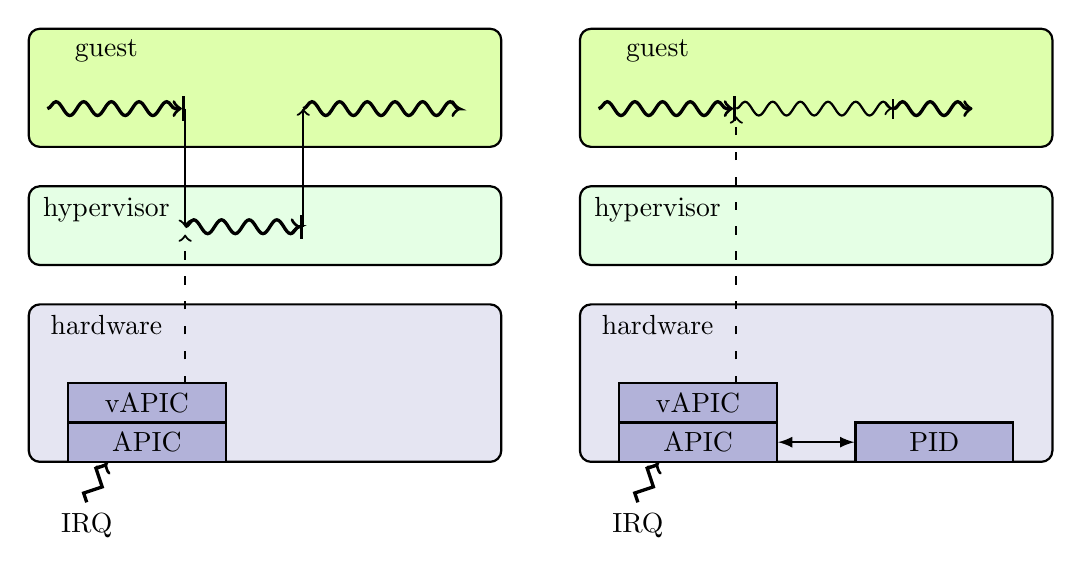
\begin{tikzpicture}


%\draw[step=0.5cm, gray, very thin] (0,0) grid (10,10);

\node at (0,0) [rectangle, draw=black, thick, rounded corners, fill=NavyBlue!10, minimum height = 2cm, minimum width = 6cm, anchor=south west] (hardware1) {} ;
\node at (1,2) [below] {hardware};
\node at (7,0) [rectangle, draw=black, thick, rounded corners, fill=NavyBlue!10, minimum height = 2cm, minimum width = 6cm, anchor=south west] (hardware2) {} ;
\node at (8,2) [below] {hardware};

\node at (0.5,0) [rectangle, draw=black, thick, fill=NavyBlue!30, minimum height = 0.5cm, minimum width = 2cm, anchor=south west] (apic1) {APIC};
\node at (7.5,0) [rectangle, draw=black, thick, fill=NavyBlue!30, minimum height = 0.5cm, minimum width = 2cm, anchor=south west] (apic2) {APIC};

\node at (0.5,0.5) [rectangle, draw=black, thick, fill=NavyBlue!30, minimum height = 0.5cm, minimum width = 2cm, anchor=south west] (vapic1) {vAPIC};
\node at (7.5,0.5) [rectangle, draw=black, thick, fill=NavyBlue!30, minimum height = 0.5cm, minimum width = 2cm, anchor=south west] (vapic2) {vAPIC};

\node at (10.5,0) [rectangle, draw=black, thick, fill=NavyBlue!30, minimum height = 0.5cm, minimum width = 2cm, anchor=south west] (pid2) {PID};

\node at (0,2.5) [rectangle, draw=black, thick, rounded corners, fill=green!10, minimum height = 1cm, minimum width = 6cm, anchor=south west] (phidias1) {} ;
\node at (1,3.5) [below] {hypervisor};
\node at (7,2.5) [rectangle, draw=black, thick, rounded corners, fill=green!10, minimum height = 1cm, minimum width = 6cm, anchor=south west] (phidias2) {} ;
\node at (8,3.5) [below] {hypervisor};

\node at (0,4) [rectangle, draw=black, thick, rounded corners, fill=GreenYellow!40, minimum height = 1.5cm, minimum width = 6cm, anchor=south west] (guest1) {} ;
\node at (1,5.5) [below] {guest};
\node at (7,4) [rectangle, draw=black, thick, rounded corners, fill=GreenYellow!40, minimum height = 1.5cm, minimum width = 6cm, anchor=south west] (guest2) {} ;
\node at (8,5.5) [below] {guest};

\draw[very thick, decorate, decoration=snake, ->|] (0.25, 4.5) -- (2, 4.5);
\draw[thick, ->] (2, 4.5) -- (2, 3);
\draw[very thick, decorate, decoration=snake, ->|] (2.0, 3) -- (3.5, 3);
\draw[thick, ->] (3.5, 3) -- (3.5, 4.5);
\draw[very thick, decorate, decoration=snake, ->] (3.5, 4.5) -- (5.5, 4.5);

\draw[thick, loosely dashed, ->] (2,1) -- (2,2.9);

\draw[very thick, decorate, decoration=snake, ->|] (7.25, 4.5) -- (9, 4.5);
\draw[thick, decorate, decoration=snake, ->|] (9, 4.5) -- (11, 4.5);
\draw[very thick, decorate, decoration=snake, ->] (11, 4.5) -- (12, 4.5);

\draw[thick, loosely dashed, ->] (9,1) -- (9, 4.4);

\draw[very thick, decorate, decoration=zigzag, ->] (0.75, -0.5) -- (1, 0) node at (0.75, -0.5) [below] {IRQ};
\draw[very thick, decorate, decoration=zigzag, ->] (7.75, -0.5) -- (8, 0) node at (7.75, -0.5) [below] {IRQ};


%\begin{scope}[fill opacity=0.9]
%	\draw[xstep=0.5cm, ystep=0.5, gray, very thin] (5,1) grid (9,5);
%\end{scope}

\begin{scope}[>=latex]
	\draw [thick, <->] (apic2.east) to [bend left=0] (pid2);
%	\draw [thick, ->] (pidaddr.center) to [bend right=45] (pir.west);
\end{scope}


\end{tikzpicture}
\end{center}
\ifreport
\caption{Comparison of virtual and direct guest interrupt delivery. 
On left, the guest interrupt is delivered to the hypervisor, and hypervisor injects the interrupt as a virtual interrupt. 
On right, interrupt is directly delivered to the guest using DII mechanism, without hypervisor involvement.}
\fi
\label{fig-pi-delivery}
\end{figure}
